\documentclass[12pt, letter, leqno]{article}
\usepackage{times,tipa}
\usepackage{
    amsmath,
    amsthm,
    amssymb,
    mathtools,
    vowel,
    geometry,
    fancyhdr,
    arydshln,
    natbib,
    graphicx,
    xcolor,
    multicol,
    multirow,
    rotating,
    pstricks,
    colortab,
    booktabs,
    tikz,
}
\usetikzlibrary{automata,positioning,arrows.meta}

\usepackage{caption}
\captionsetup{font=it,justification=centering}

\usepackage{multicol, multirow, endnotes, tree-dvips}

\renewcommand\floatpagefraction{.9}
\renewcommand\topfraction{.9}
\renewcommand\bottomfraction{.9}
\renewcommand\textfraction{.1}   
\setcounter{totalnumber}{50}
\setcounter{topnumber}{50}
\setcounter{bottomnumber}{50}

\raggedbottom

\usepackage[small,compact]{titlesec}

\usepackage[Symbolsmallscale]{upgreek} 

\titleformat*{\section}{\normalsize \bf}
\titleformat*{\subsection}{\normalsize \bf}
\titleformat*{\subsubsection}{\normalsize}
%
%\renewcommand{\footnotesize}{\normalsize}

\geometry{letterpaper, left=1in,right=1in,top=1in,bottom=1in}

\usepackage{setspace}
\doublespacing

\usepackage[singlelinecheck=off]{caption}


\usepackage{tree-dvips}

\usepackage{soul}

% \usepackage{gb4e}  % IMPORTANT: should be the last \usepackage
\usepackage{lingmacros}  % not to be confused with ling-macros

% bmatrix is a bit too big
% i packaged this out because it messed up my syntax highlighting
\newenvironment{setmatrix*}[1][c]
    {\renewcommand{\arraystretch}{0.6}
        \left\{%
        \begin{matrix*}[#1]}
    {\end{matrix*}\right\}}

\newenvironment{featmatrix*}[1][c]
    {\renewcommand{\arraystretch}{0.6}
        \left[%
        \begin{matrix*}[#1]}
    {\end{matrix*}\right]}


\frenchspacing

\newcommand{\sz}{\v}     

\newtheorem{theorem}{Theorem}
\newtheorem{definition}{Definition}

\begin{document}
        
\begin{center}
\textbf{
    Opacity in Chumash Restricts Possible Phonotactics
}

% NOTE: Alt title: Multi-tiered Strictly Local Functions and Opacity in Chumash

Leo Peckham

\end{center}

% TODO: double check formatting instructions

\section{Introduction}

If you're reading this, there are a lot of comments in the LaTeX that you're
missing by just reading the PDF!

% NOTE: This project has taken flight! I still have a feeling that I'm behind
% the rest of the class, but after scrapping 5 or 6 analyses, and staying up
% until well past 3am, I am confident that not only is this current analysis
% correct, but significant. That being said, this document is currently very
% unpolished. As well as completing all of the TODOs littered throughout the
% document, I also still have some major sections to write, and fill out every
% missing citation.
%
% The rest of the documents in this repository probably need updating as well.

% TODO: Save the best for last!

\section{Linguistic motivation}

\citet{mcnaughton&papert71} introduced Strictly Local (SL) languages as a
theory of phonotactics, aiming to explain what types of well-formedness
judgments can exist in natural language. Many phonotactic patterns are SL, and
have seen a great deal of success theoretically, as well as achieving some
strong learnability results \citep{garcia+90,heinz10a,heinz10b,heinz&rogers13}.
Strict Locality was extended to \textit{Input} Strict Locality (ISL) and
\textit{Output} Strict Locality (OSL) in \citet{chandlee14}, which provides a
much stronger formalism. An important property of ISL for this paper is that a
wide range of phonologically opaque maps are ISL \citep{chandlee+18}. SL
languages, however, fail to account for long-distance dependencies.

% TODO: provide example of long-distance dependency that SL fails to account
% for

Various ways to account for this deficiency have been proposed.
\citet{rogers+10} introduced Strictly Piecewise (SP) languages, which are also
efficiently learnable, but still fail to describe some long-distance patterns
\citep{cook84}. The Strict Locality \citep{gafos99} hypothesis simply suggests
that long-distance dependencies of this type simply do not exist, and are
simply feature spreading, with the spread feature being imperceptible on most
segments. There is some phonetic evidence for this perspective
\citep{walker+09,gafos99}, but this hypothesis is contrary to \citet{hansson01}
and \citet{rose&walker04}, and there remain issues with learnability.

% TODO: provide example of how the strict locality hypothesis would handle this

A stronger framework is that of Tier-based Strictly Local (TSL) languages
\citep{heinz+11}, based on the idea of the phonological tier \citep{goldsmith76}.
TSL languages keep all of the advantages of SL languages (learnability,
theoretical results), while also succeeding in handling long-distance
dependency
\citep{jardine&heinz16,burness&mcmullin19,mcmullin&hansson15,heinz+11}.

% TODO: discuss how tiers are normally described, and the extension in
% mutli-tier strictly local languages

In particular, \citet{burness&mcmullin19} extend Tier-based Strict Locality by
combining it with Input and Output Strict Locality \citep{chandlee14}. In their
paper, they describe Output Tier-based Strictly 2-Local functions, but the
definition for Input Tier-based Strictly $k$-Local functions (which we will use
in this paper) is constructed similarly.

We use TSL functions to describe the opacity in this paper because of their
learnability results. Opaque patterns are learnable \citep{?}, but not
trivially. So, to be able to work with opacity, it is useful to work within a
theory that has learnability results. Rule-based approaches (and the regular
languages they describe) fail to be learnable in generale \citep{?}. Optimality
theory (OT) also struggles with learnability in opacity \citep{?} as well as
its other well-known issues \citep{?}.

\section{Mathematical preliminaries}

% TODO: on this whole section

Defitions based on \citet{chandlee14} and \citet{burness&mcmullin19}. I do not
know exactly what I will need yet, but probably: ISL, some formal language
theory, TSL functions, transducers, and some relational theorems.

Normally (cite who), OSL functions are chosen to deal with harmony, because ISL
functions simply cannot handle it, but with ITSL we no longer need to make this
concession.

% TODO: Needs work.
We typically do the definition as left-to-right maps, indeed this is how
\citet{chandlee14} defines ISL, however, we can just as easily define
right-to-left maps. In this paper, we will present and use the right-to-left maps. For more discussion of left-to-right maps and switching direction see \citet{chandlee14} and \cite{heinz&lai13}.

\citep{chandlee14} and \citep{heinz&lai13} show how ISL functions can be
transformed to work on right-to-left processes as well. Since the definitions
are so similar we will only consider left-to-right processes in this paper.

\section{Properties of ITSL functions}

\begin{figure}[h]
    \centering
    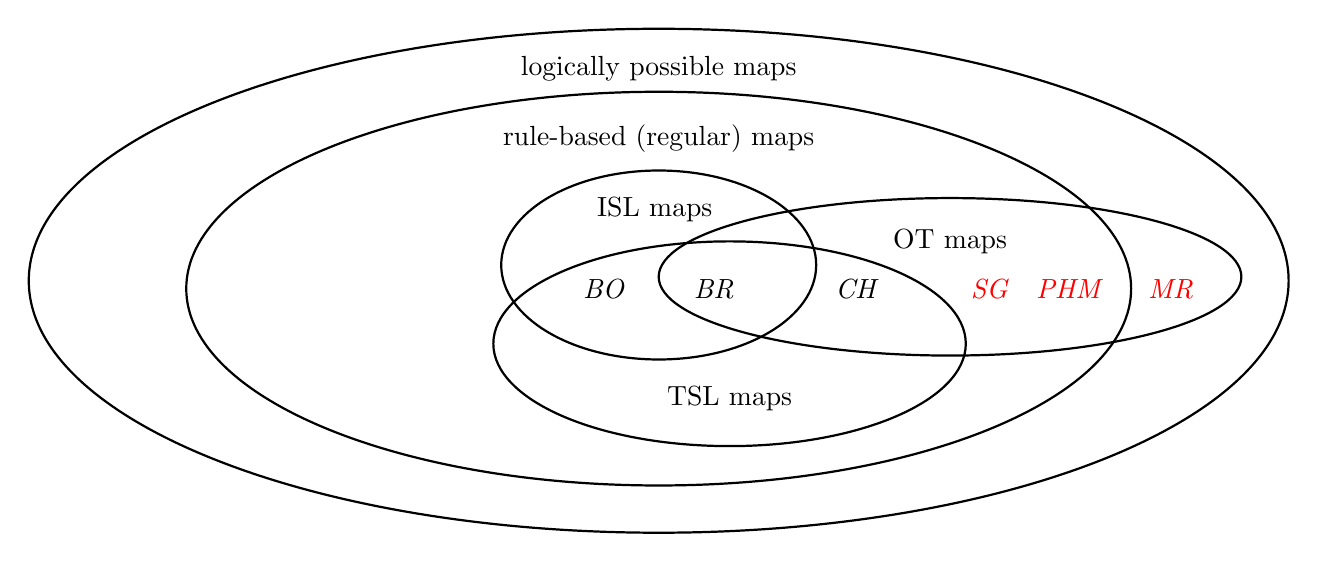
\begin{tikzpicture}[scale=1]

    \draw[thick] (0,-0.2) ellipse (8 and 3.2);
    \node at (0,2.5) {logically possible maps};

    \draw[thick] (0,-0.3) ellipse (6 and 2.5);
    \node at (0,1.6) {rule-based (regular) maps};

    \draw[thick] (0,0) ellipse (2 and 1.2);
    \node at (-0.05, 0.7) {ISL maps};

    \draw[thick] (3.7,-0.15) ellipse (3.7 and 1);
    \node at (3.7, 0.3) {OT maps};

    \draw[thick] (0.9,-1) ellipse (3 and 1.3);
    \node at (0.9, -1.7) {TSL maps};

    \node at (-0.7,-0.3) {\it BO};
    \node at (0.7, -0.3) {\it BR};
    \node at (2.5, -0.3) {\it CH};
    \node[color=red] at (4.2, -0.3) {\it SG};
    \node[color=red] at (5.2, -0.3) {\it PHM};
    \node[color=red] at (6.5, -0.3) {\it MR};

    \end{tikzpicture}
    \caption{
        Parts of the subregular hierarchy and their accompanying theories
        (regular text) as well as their predictions (italics) of different
        types of patterns. Unattested patterns are highlighted in red.
        (BO=Bedouin opacity; BR=Bedouin raising; CH=consonant harmony; SG=sour
        grapes harmony; PHM=Poser; Hansson and McCarthy opacity (see section
        \ref{phm}); MR=majority rules harmony) See \citet{chandlee+18} and
        \citet{prickett22}.
    }
    \label{fig:hierarchy}
\end{figure}

% TODO: Discuss figure \ref{fig:hierarchy}.
% TODO: Discuss previous known results about TSL and opacity

\section{Chumash}

Chumash, was an isolate language in California, now extinct. The language has
two main dialects of interest, the Inezeño dialect and the Ventureño
dialect. The first grammar of Chumash was \citeauthor{applegate72}'s
\citeyearpar{applegate72} thesis, based on Harrington's field notes on the
Inezeño dialect. A description of the Ventureño dialect was posthumously
published as Harrington (1974). The dialects are very similar, and most papers
on the language focus primarily on the Inezeño dialect. When we refer to
Chumash in the rest of this paper, we are referring to the Inezeño dialect.

\subsection{Sibilant $[$anterior$]$ harmony}

Chumash features two interacting rules\footnote{ The $[\pm$anterior$]$ affricate
pair \textipa{/ts/} and \textipa{/tS/} undergo the same rules, but there is
more variation. We will not consider these phonemes for this paper. } that we
care about: $[$anterior$]$ dissimilation in sibilant-dental clusters, and
long-distance $[$anterior$]$ harmony on its sibilants.

% TODO: Present consonant inventory, and some of the important natural classes

\enumsentence{
    Dissimilation\label{ex:dissimilation} \citep[pp.~115,117]{applegate72}
    \vspace{-1em}
    \begin{tabbing}
        \hspace*{1em} \= \hspace*{6em} \= \hspace*{5em} \= \kill
        \>\textipa{/s+kal+w1j/} \> \textipa{[skaw'1j]}
            \> `he cuts a notch in it'\\
        \>\textipa{/s+tepuP/} \> \textipa{[StepuP]} \> `he gambles'\\
        \>\textipa{/s+niP/} \> \textipa{[SniP]} \> `his neck'\\
        \>\textipa{/s+lok'in/} \> \textipa{[Slok'in]} \> `he cuts it'
    \end{tabbing}
}

\enumsentence{
    Rule-based analysis of dissimilation\label{rule:dissimilation}
    \begin{multline*}
        \begin{featmatrix*}[l] 
            +\text{ant}\\
            +\text{cor}\\
            +\text{strid} 
        \end{featmatrix*}  
        %
        {\rightarrow} 
        %
        \begin{featmatrix*}[l] 
            -\text{ant}
        \end{featmatrix*} 
        \Big/
        \underline{\hspace{0.5cm}} 
        %
        {~+}
        \begin{featmatrix*}[l] 
            +\text{cons} \\
            +\text{ant} \\
            +\text{cor} \\
            +\text{strid}
        \end{featmatrix*} 
    \end{multline*}
}

The data in (\ref{ex:dissimilation}) shows the process of dissimilation in
Chumash, with the rule given in (\ref{rule:dissimilation}). Notably, Chumash
dissimilation only happens around morpheme
boundaries\footnote{\citet{applegate72} describes two different types of
morpheme boundaries in Chumash, close ($=$) and remove ($+$), but does not
distinguish between them for the present analysis.} \citep{applegate72}. For
the purposes of this paper, (\ref{rule:dissimilation}) is just
$\text{\textipa{s}} \rightarrow \text{\textipa{S}} \big/
\underline{\hspace{0.3cm}} {+} \{\text{\textipa{t, n, l}}\}$.

% TODO: Say a bit more when we have the consonant inventory

\enumsentence{
    Harmony\label{ex:harmony} \citep[pp.~72,119,272]{applegate72}
    \vspace{-1em}
    \begin{tabbing}
        \hspace*{1em} \= \hspace*{10em} \= \hspace*{8em} \= \kill
        \>\textipa{/s+xalam+S/} \> \textipa{[SxalamS]} \> `it is wrapped'\\
        \>\textipa{/k+s1p1t+waS/} \> \textipa{[kS1p1twaS]}
            \> `I made acorn mush'\\
        \>\textipa{/waS+mas1x/}\footnote{$[+$anterior$]$ harmony seems to be
            much rarer than $[-$anterior$]$ harmony. Without a living native
            speaker, this is cause for concern, but ultimately I do not feel
            it affects the analysis.} \> \textipa{[wasmas1x]}
            \> `to be triple-ply'\\
        \>\textipa{/s+taja+nowon+waS/} \> \textipa{[StojonowonwaS]}
            \> `it stood upright'
    \end{tabbing}
}

\enumsentence{
    Rule-based analysis of harmony\label{rule:harmony}
    \begin{multline*}
        \begin{featmatrix*}[l] 
            +\text{cor}\\
            +\text{strid} 
        \end{featmatrix*}  
        %
        {\rightarrow} 
        %
        \begin{featmatrix*}[l] 
            \alpha\text{ant}
        \end{featmatrix*} 
        \Big/
        \underline{\hspace{0.5cm}} 
        %
        \begin{setmatrix*}[l] 
            C \\
            V \\
            +
        \end{setmatrix*}_0
        \begin{featmatrix*}[l] 
            \alpha\text{ant} \\
            +\text{cor} \\
            +\text{strid}
        \end{featmatrix*} 
    \end{multline*}
}

% TODO: check if I'm saying interesting. Don't
% TODO: actually, go back through that slideshow and just check off things
% TODO: check for \cite that are not \citet or \citep

The harmony we observe in (\ref{ex:harmony}) has been of particular interest in
the literature as an example of long-distance harmony. This type of harmony,
that spreads on a very narrow tier, and can spread over morpheme boundaries, is
rare crosslinguistically \citep{?}, and poses some big problems to popular
theories. It is neither SL or ISL, and both OSL and TSL languages were in part invented just to deal with patterns like these \citep{chandlee14,heinz+11}. 

\enumsentence{
    Dissimilation and harmony opacity\label{ex:interaction}
    \citep[pp.~119--120]{applegate72}
    \vspace{-1em}
    \begin{tabbing}
        \hspace*{1em} \= \hspace*{7em} \= \hspace*{5em} \= \kill
        \>\textipa{/s+uSla+s1q/} \> \textipa{[suslas1q]}
            \> `he presses it tight' \\
        \>\textipa{/s+is+t1P/} \> \textipa{[SiSt1P]} \> `he finds it' \\
        \>\textipa{/s+net+us/} \> \textipa{[snetus]} \> `he does it to him'
    \end{tabbing}
}

% TODO: Check all \refs for ()

The data in (\ref{ex:interaction}) shows these rules interacting in a pattern
that looks exactly like \textit{fed counterfeeding on focus} (sometimes called
a \textit{Duke of York derivation}) \citep{bakovic11}, which suggests that
dissimilation is ordered before harmony. Indeed, this is what
\citet{applegate72} proposes, and explains the vast majority of the data. This
opacity was even shown to be productive, applying to loan-words
\citep{applegate72}. However, there are also a few known exceptions, given in
(\ref{ex:noundergo}).

\enumsentence{
    Output of dissimilation does not undergo harmony\label{ex:noundergo}
    \citep[pg.~120]{applegate72}
    \vspace{-1em}
    \begin{tabbing}
        \hspace*{1em} \= \hspace*{8em} \= \hspace*{6em} \= \kill
        \>\textipa{/s+ti+jep+us/} \> \textipa{[Stijepus]} \> `he tells him' \\
        \>\textipa{/s+iS+lu+sisin/} \> \textipa{[SiSlusisin]}
            \> `they (dual) are grown awry'
    \end{tabbing}
}

\subsection{Poser, Hansson and McCarthy's analysis} \label{phm}

% TODO: none of these analyses include s+net+us... why?

There have been several attempts to justify the exceptions in
(\ref{ex:interaction}), each building on another
\citep{poser82,poser93,hansson01,mccarthy07}. However, \citet{heinz&idsardi10}
revealed through personal communication with Applegate, that instances like
those in (\ref{ex:interaction}) are not \textit{type} exceptions but
\textit{token} exceptions, and they pare rare (less than roughly 5\%). There
are many ways to account for variation like this\footnote{Given the prevalence
of morpheme boundary rules, and the distinction between close and remote
morpheme boundaries, I hypothesize that the sibilant harmony variably gets
blocked by close boundaries. That being said, any theory of variation is
exceedingly hard to test without any living native speakers}, but this type of
pattern being a phonological \textit{rule} is unlikely.


% NOTE: I don't really know what to call this section? Discussion seemed the
% most appropriate

% TODO: switch the whole analysis around, we need to use MTSL functions!

\section{Discussion}

We would now like to take a closer look at the analysis used by Poser, Hansson
and McCarthy (PHM), and show that exceptions that motivated their analysis are
not only incorrect in Chumash, but form a pattern that is impossible for an
entire class of languages like Chumash under a MTSL framework. We will then
relax our defining constraints of this class of languages to show their
necessity. Finally, we will argue that because MTSL satisfies properties we
expect to be true of any well-formed phonological theory, that this result
extends far beyond the scope of MTSL.

\subsection{PHM opacity}

Motivated by the Chumash data and subsequent analysis, we prose naming this
particular subset of fed counterfeeding on focus opacity \textit{PHM opacity},
and we will call any language that has PHM opacity a \textit{PHM opaque
language}. Precisely, PHM opacity requires:

\begin{enumerate}

    \item Two tiers: $\Theta_\mathbb{B}$, which includes at least two segments
        $T$ and $S$; and $\Theta_\mathbb{A}$, which is a strict superset of
        $\Theta_\mathbb{B}$.

    \item A process $\mathbb{A}$ able to create $T$ from $S$ on the tier
        $\Theta_\mathbb{A}$.

    \item A long-distance harmony process\footnote{This does not need to be a
        symmetric process like it is in Chumash} $\mathbb{B}$ able to create
        $S$ from $T$ on the tier $\Theta_\mathbb{B}$.

    \item There is some $e \in \Theta_\mathbb{A} - \Theta_\mathbb{B}$ such that
        there can be arbitrarily many instances of $e$ between any two segments
        in $\Theta_\mathbb{B}$. 

    \item $\mathbb{A}$ feeds $\mathbb{B}$ but $\mathbb{B}$ in turn counterfeeds
        $\mathbb{A}$ (fed counterfeeding on focus).

    \item The opaque interaction is productive.

\end{enumerate}

This is exactly fed counterfeeding on focus with the additional requirements
that the feeding process is long-distance harmony, and that the opacity is
productive.

We already know the combination of Chumash harmony and dissimilation to be MTSL
from \citet{burness&mcmullin20}, but now we want to show that this is true in
general for PHM opacity.

\begin{theorem}
    PHM opaque languages are MTSL.
\end{theorem}
\begin{proof}
    % TODO: not the most important result, since we know Chumash is, and this
    % seems pretty obvious from that data, but not trivial to prove! definitely
    % something I'll have to write before the final submission
\end{proof}

Now we want to describe the types of exceptions that we expect to be illegal in
a PHM opaque language. Consider again the problematic Chumash word
\textipa{/s+iS+lu+sisin/} $\rightarrow$ \textipa{[SiSlusisin]}. For this to be
an MTSL map, we would need (at least) to keep on one tier $\tau_1$ the vowels,
morpheme boundaries, and sibilants, and on another tier $\tau_2$ just the
sibilants. Since $\tau_2 \subseteq \tau_1$, these are valid MTSL tiers. We use
$\tau_1$ to do dissimilation, and $\tau_2$ to do harmony. Now consider the fact
that if instead of having \textipa{/iS+lu/} (which blocks harmony), there was
no morpheme boundary and we just had \textipa{/iSlu/}. This would allow the
harmony to pass through, but without changing any features of the sibilant.
Since $\tau_1$ is the superset, the only way for the morpheme boundary to
interact with the harmony rule is by changing features on the sibilant. This
means that the harmony rule has no way of recognizing that it's supposed to
pass through. We cannot fix this by making harmony aware of any other useful
segments without violating the constraints on MTSL tiers. Therefore, this word
is not compatible with PHM opacity in Chumash.

To formalize this intuition, an underlying form $w$ is \textit{not allowed} in
a PHM opaque language if:

\begin{enumerate}

    \item There is some substring $u$ of $\text{erase}_\mathbb{A}(w)$ that
        blocks $\mathbb{A}$.

    \item There is a segment $e$ in $u$, such that $e$ is not a member of
        $\mathbb{B}$, and there can be arbitrarily many instances of $e$
        between any two segments in $\mathbb{B}$.

    \item $\text{erase}_\mathbb{B}(u)$ does not block $\mathbb{A}$.

\end{enumerate}


\begin{theorem}
    PHM opaque languages are MTSL.
\end{theorem}
\begin{proof}
    % TODO: another proof I need to write before submission. I hope this one is
    % also clear just from the example above.
\end{proof}

\subsection{Why not TSL?}

Chumash (and other PHM opaque languages) is \textit{not} TSL. To see this,
consider the (hypothetical) word \textipa{/sa+(ka+)$^*$s+ta/}. If we choose our
tier to be \textipa{/s/}, \textipa{/S/}, and \textipa{/t/}, then we incorrectly
guess the form \textipa{/Sa+(ka+)$^+$S+ta/}, so we need to also include the
morpheme boundary in our tier. However, if we include the morpheme boundary,
then we would have an arbitrary number of morpheme boundary segments between
the two sibilants from the morpheme \textipa{/+ka+/}. This prevents Chumash
from being TSL.

% NOTE: I have some FSTs in another file showing that each rule is TSL in their
% own right. Is that worth including? This also shows that TSL is not closed
% under composition, which is a neat finding. 

Another option would be to simply consider both dissimilation and harmony rules
independently, since they are each TSL on their own. This does not work,
because to show that the opaque interaction is learnable, we require the entire
language (or subset of the language that creates the opaque interaction) to be
a single formalism with a learning guarantee. This is why we need to use MTSL
instead of TSL.

\subsection{Relaxing constraints}

% TODO: talk about why we cant use several rules sequentially. viz.

\subsection{Other opaque patterns}

\subsection{Theory-independence}

% - Describe the types of long-distance opactiy ISL couldn't handle, then show
%   that these are ITSL as compositions of other ITSL functions
% - Discuss Learnability

\section{Conclusion}

\section*{Acknowledgments}


\bibliography{bib}
\bibliographystyle{linquiry2}

\end{document}
